\documentclass[12pt,a4paper]{article}
\usepackage{graphicx}
\usepackage{hyperref}
\usepackage{amsmath}
\usepackage{float}

\begin{document}

\title{File transfer process in Peer-To-Peer networks}
\author{Le Viet An}
\date{December, 2024}
\maketitle

\tableofcontents
\newpage

\section{Introduction}

Peer-to-Peer (P2P) networks have revolutionized the way resources are shared and accessed in distributed systems. Unlike traditional client-server architectures, P2P networks allow peers to act as both clients and servers, enabling decentralized communication and resource sharing. This report explores the concept of P2P networks and the detailed process of file transfer within such networks.

\section{Concept of Peer-to-Peer Networks}

A P2P network is a distributed system where each participant, referred to as a peer, can communicate directly with other peers. In this network architecture, peers share resources such as files, bandwidth, and processing power without relying on a central server.

\subsection{Characteristics of P2P Networks}
\begin{itemize}
    \item \textbf{Decentralization:} There is no central authority or server managing the network.
    \item \textbf{Scalability:} The network grows and becomes more robust as more peers join.
    \item \textbf{Resource Sharing:} Each peer contributes resources to the network.
    \item \textbf{Fault Tolerance:} The failure of one or more peers does not disrupt the entire network.
    \item \textbf{Dynamic Participation:} Peers can join or leave the network at any time.
\end{itemize}

\subsection{Types of P2P Networks}
\begin{itemize}
    \item \textbf{Pure P2P:} All peers have equal roles, and there is no central server.
    \item \textbf{Hybrid P2P:} Includes a central server for peer discovery but uses direct peer-to-peer communication for resource sharing.
    \item \textbf{Structured P2P:} Utilizes distributed hash tables (DHTs) for efficient resource lookup.
    \item \textbf{Unstructured P2P:} Peers connect randomly, making resource lookup less efficient but simpler.
\end{itemize}

\section{File Transfer Process in P2P Networks}

File transfer in P2P networks involves the direct exchange of files between peers without intermediary servers. This process is often faster and more efficient than traditional file-sharing methods. Below is a detailed explanation of the file transfer process in a P2P network.

\subsection{Step-by-Step File Transfer Process}
\begin{enumerate}
    \item \textbf{Peer Discovery:}
    A peer seeking a file must first discover other peers in the network. This can be achieved through methods such as:
    \begin{itemize}
        \item Bootstrapping servers: Temporary servers that provide a list of active peers.
        \item Broadcasting: Sending a discovery request to all peers in the network.
        \item Distributed Hash Tables (DHTs): A decentralized mechanism to locate peers with the required file.
    \end{itemize}

    \item \textbf{File Search:}
    The requesting peer sends a query to the network to locate the desired file. Depending on the network type, the query can be flooded to all peers or targeted using DHTs.

    \item \textbf{Connection Establishment:}
    Once the file’s location is identified, the requesting peer establishes a direct connection with the peer(s) hosting the file.

    \item \textbf{File Download:}
    The file is downloaded using a transfer protocol such as:
    \begin{itemize}
        \item TCP (Transmission Control Protocol): Ensures reliable and complete file transfer.
        \item UDP (User Datagram Protocol): Faster but less reliable, suitable for real-time applications.
    \end{itemize}
    Files may be:
    \begin{itemize}
        \item Downloaded entirely from a single peer.
        \item Split into smaller chunks and downloaded from multiple peers simultaneously (e.g., BitTorrent protocol).
    \end{itemize}

    \item \textbf{Data Verification:}
    Each downloaded file or chunk is verified using hash functions to ensure data integrity. If a chunk is corrupted, it is re-requested from the network.

    \item \textbf{Sharing (Seeding):}
    After downloading, the peer becomes a seeder, sharing the file or chunks with other peers requesting it.
\end{enumerate}

\begin{figure}[H]
    \centering
    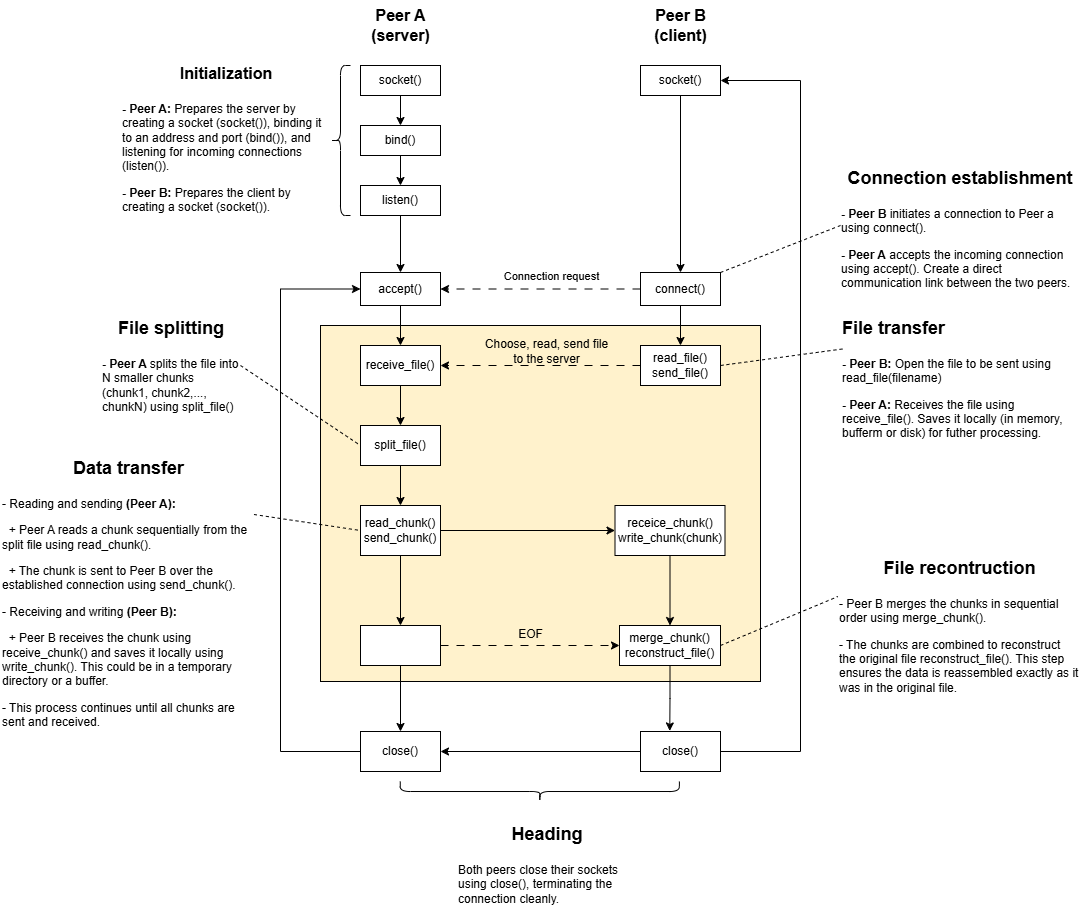
\includegraphics[width=\textwidth]{A-P2P-file-sharing-application-system.png}
    \caption{Illustration of Peer-to-Peer Network File Transfer Process}
    \label{fig:p2p-transfer}
\end{figure}

\section{References}

\begin{enumerate}
    \item \href{https://www.brosix.com/blog/peer-peer-file-transfer/}{Brosix: Peer-to-Peer File Transfer}
    \item \href{https://www.geeksforgeeks.org/p2p-peer-to-peer-file-sharing/}{GeeksforGeeks: P2P File Sharing}
    \item \href{https://www.raysync.io/news/everything-you-need-to-know-about-point-to-point-transfer/}{Raysync: Point-to-Point Transfer}
    \item Andrew S. Tanenbaum, "Computer Networks," 5th Edition.
    \item BitTorrent Protocol Specification.
    \item Peer-to-Peer Network Design and Applications.
\end{enumerate}

\end{document}
